\documentclass{scrartcl}
\usepackage[utf8]{inputenc}
\usepackage[english]{babel} % Trennung nach der neuen deutschen Rechtschreibung
\usepackage[utf8]{inputenc}
\usepackage[T1]{fontenc}
\usepackage{lmodern}
\usepackage[dvipsnames]{xcolor}
\usepackage{hyperref}
\definecolor{Mycolor2}{HTML}{f8f8ff}
\definecolor{RickBoy}{HTML}{ff1a1a}

\usepackage{amsmath} % Erweiterte Mathematik-Umgebung
\usepackage{amsfonts} % zusätzliche Mathematik-Schrifttypen (v.a. \mathbb für Mengen)
\usepackage{ulem}

\usepackage{graphics}%soll beim Graphiken einfügen hilfreich sein
\usepackage{graphicx}
\usepackage{wrapfig}%lässt Textumflossene Bildeinbindung zu
\usepackage{epstopdf}%soll eps in pdf umwandeln

\usepackage[a4paper, portrait, margin=2.5cm]{geometry}

\titlehead{\centering University of Luxemburg}
\subject{Travaux Pratiques}
\title{Interferometry}
\subtitle{ }
\date{TP Session 03/12/2021}
\author{Louis-Hendrik Barboutie (020157041C)\\ Frederik Ehl (0201719742) \\ Florence Schmerber (0201845640)}

\begin{document}

\maketitle

\clearpage

\tableofcontents

\listoffigures
	
\clearpage

\section{Introduction}
In todays TP, we are interested in the interference of light. The superposition of two waves results in either constructive or destructive interference, where the former can be seen when the two waves are in phase and their amplitudes add up, and the latter, as the name describes, when they're out of phase of 180° and their amplitudes cancel each other out. In order to observe this phenomenon we use an interferometer, in our case the Michelson Interferometer. This apparatus creates a phase shift of an incoming source of light, by splitting the light ray with a beam slitter. As the two resulting beams come from the same source, we can say that they are coherent waves, who have the ideal properties for inference by having the same waveform and the same frequency.
%The aim of this TP is to measure the the difference in distance

\section{Experimental setup}
We will use the Mickelson Interferometer. This apparatus consist of a swappable laser, a lens, two mirrors, one movable and the other one adjustable and a beam splitter. The incoming light goes through the lens, such that it expands the light in order to see interference in the first place, and will be split in two by hitting the beam splitter. One ray goes to mirror $M_1$ and the second to mirror $M_2$. When they are reflected back, they meet again, but since they travelled different distances we can observe constructive and destructive interference. 
We will also use a vacuum cell, where we can change the pressure which will alter the refractive index $n$. 
At the end of this experiment we will briefly use two polarizers that are placed in front of $M_1$ 
and $M_2$ to observe the effects on the interference pattern.

\begin{figure}[h]
    \centering
    \includegraphics[width= 10cm]{Screenshot 2021-12-03 090339.png}
    \caption{Mickelson Interferometer setup}
    \label{fig:my_label}
\end{figure}

\section{Results}
\subsection{Preliminary preparation}
We first align the laser. Therefore we remove the beam splitter and attach a glass plate at the entrance of the interferometer. We make sure that the laser hits the glass plate in it's center and that the reflection by the movable mirror $M_1$ overlaps with the initial laser beam. We also make sure that the entire setup is leveled using a spirit level.
We then set up the Michelson mode, which means, we introduce the beam splitter at an angle of $45^\circ$ and remove the glass plate. At this point we can observe two sets of bright spots on the screen, each consisting of a bright dot and a couple of darker spots. This is due to the fact that the the beam splitter acts as a prism and therefore defracts the light. 
We then attach the lens to the entrance of the interferometer and adjust it in a way, that the beam is centered on the beam splitter. We now can observe circular fringes on the screen.

%why not turn in the other direction -> spring and it takes some time to readapt.

\subsection{Calibrating the micrometer}
In order to calibrate the micrometer, we want to count the fringes we can observe( red circles) while turning the micrometer.
 We count at least 30 fringes and take the reading on the micrometer (we note the starting position, in our case 0,5mm and the final reading after we've counted at least   30 fringes) We do this for k=30, k=40 and k=50. With those measurements and using the relation $\Delta I_{micrometer}= 2(m_2-m_1)$, $m_1$ being the starting point and $m_2$ the final position and calculate the average and error on qtiplot.
 Then we calculate the true change of the optical path using: $\Delta l= k \cdot \lambda$. The wavelength of the red laser is given in the TP script and has a value of $\lambda = 632 nm$. Finally we calculate the ratio between the two $\frac{\Delta l}{\Delta l_{micrometer}}$
 We get:
 
\medskip
\centering
\begin{tabular}{|c|c|c|c|c|}
    \hline
     k & $m_2$ in m & $\Delta l_{micrometer}$ in m & $\Delta l$ in m & ratio\\
     \hline
     $30$ & $6,59 \cdot 10^{-5}$ & $3,18 \cdot 10^{-5}$ & $1,90 \cdot 10^{-5}$ & 0,60 \\
     \hline
     $35$ & $7,1 \cdot 10^{-5}$ & $4,20 \cdot 10^{-5}$ & $2,21 \cdot 10^{-5}$ & 0,53 \\
     \hline
     $40$ & $6,97 \cdot 10^{-5}$ & $3,94 \cdot 10^{-5}$ & $2,53 \cdot 10^{-5}$ & $0,64$ \\
     \hline
     $45$ & $7,3 \cdot 10^{-5}$ & $4,6 \cdot 10^{-5}$ & $2,84\cdot 10^{-5}$ & $0,62$ \\
     \hline
     $50$ & $7,45 \cdot 10^{-5}$ & $4,9 \cdot 10^{-5}$ & $3,16 \cdot 10^{-5}$ &  $0,65$\\
     \hline
    \end{tabular}
\flushleft

The avergae value we get for the ratio is then $(\frac{\Delta l}{\Delta l_{micrometer}})_{avg} = 0,61$

\subsection{Influence of polarisation}
In this part of the experiment we add polarizers in front of both mirrors. We can still observe an interference pattern on the screen, although it does no longer consist of concentric circles. When we turn one polarizer by $90^\circ$ relative to the other, the interference pattern disappears. 

\subsection{Refractive index of air}
Now we'll make use of the vacuum cell. We will change the pressure inside the cell with a pressure pump and observe a change in the interference fringes. The light travels faster in vacuum and thus the change in refractive index can therefore be related to the number of fringes we observe.
Additionally the relation between the refractive index and pressure is:

\begin{equation}
    n= 1+ \Gamma \cdot p
\end{equation}

With $\Gamma$ being a coefficient depending on the polarisability of the molecule.

But for a small change in n we get:

\begin{equation}
    \Delta n= \Gamma \Delta p = \frac{\lambda}{2d}k
\end{equation}

Where d=3cm
If we rearrange this equation we get:

\begin{equation}
    k= \frac{2d}{\lambda}\Gamma \Delta p
\end{equation}

Here $\Delta p= p_{atmos}-p_{pump}$ and the actual atmospheric pressure in Luxembourg is $p_{atmos} = 1,009\cdot10^5 Pa$ according to \href{https://www.youtube.com/watch?v=dQw4w9WgXcQ}{kachelmannwetter.com} \textcolor{RickBoy}{(click me)}.

To find the refractive index, we count the number of fringes while we change the pressure of the cell and plot the results on QtiPlot.
The slope of the linear fit describes $\frac{2d}{\lambda} \Gamma$
\newline
We find $\frac{2d}{\lambda} \Gamma = 2,038 \cdot 10^{4} Pa^{-1}$, from which we seduce $\Gamma = 0,21 Pa^{-1}$ %3,4.10^{-9}$.

\begin{figure}[ht]
    \centering
    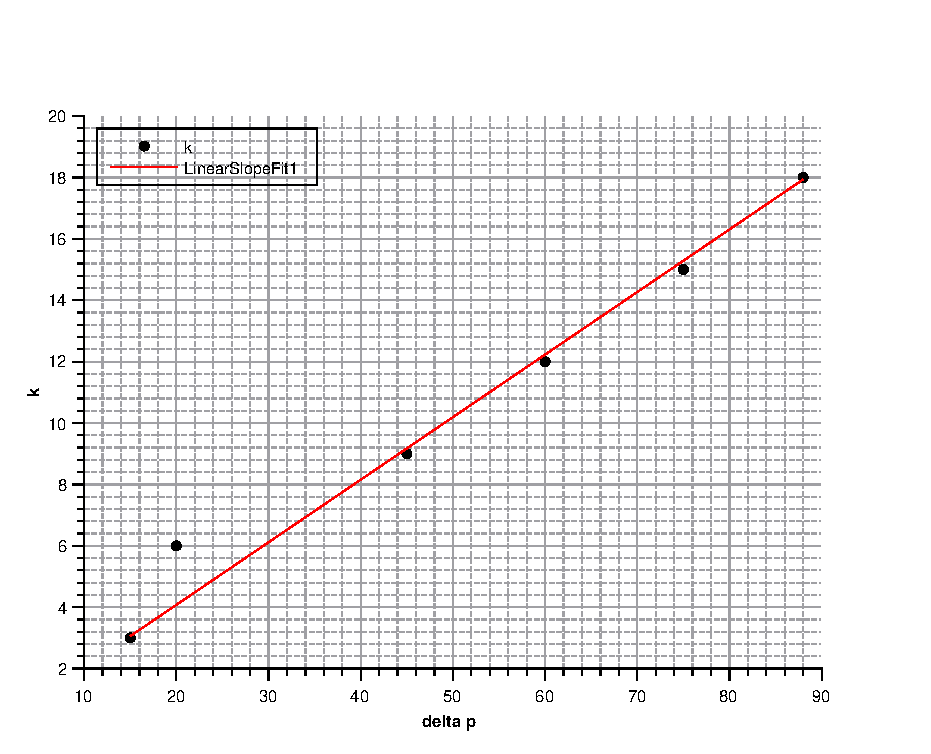
\includegraphics{gammGraph.eps}
    \caption{k as a function of $\Delta p$}
    \label{fig:my_label}
\end{figure}


\subsection{Wavelength of the green laser}
In this final part of the experiment our goal is to find out the unknown wavelength of the green laser. In order to calculate it, we use the coefficient (average ratio) we found in the first part of this TP and use the relation:

\begin{equation}
    \lambda= \frac{2(m_2-m_1)}{k} \cdot \frac{\Delta l}{\Delta l_{micrometer}}
\end{equation}

Using $m_1 = 500 \mu m$ and $m_2 = 521 \mu m$, we get $\lambda = 512,4nm$. This corresponds to smexy green light, just as for our laser. We can estimate the relative error to the actual value of 532nm: we have a relative error of 3,76\%. 
% for the wavelength, which is yellow, not green but whatever i don't give a shit. \textcolor{Mycolor2}{I'm colorblind anyways, this is fucking discriminating}
\section{Conclusion}
In the first part of the experiment we determined the calibration of the micrometer to later determine the wavelength of an unknown laser.
We found that the laser was, in fact and big surprise, green. We got this result with relatively low deviation, despite the rudimentary measuring methods and the unknown unit of the micrometer, which we eliminated by introduction the ratio with the optical path length.
We also determined $\Gamma$, which describes the dependency of the refractive index 
of gases from the atmospheric pressure. 

\centering



Happy Holidays

%FUCK OFF!

\end{document}